\begin{frame}{Random shapes, sizes, angles and brightness}
\centering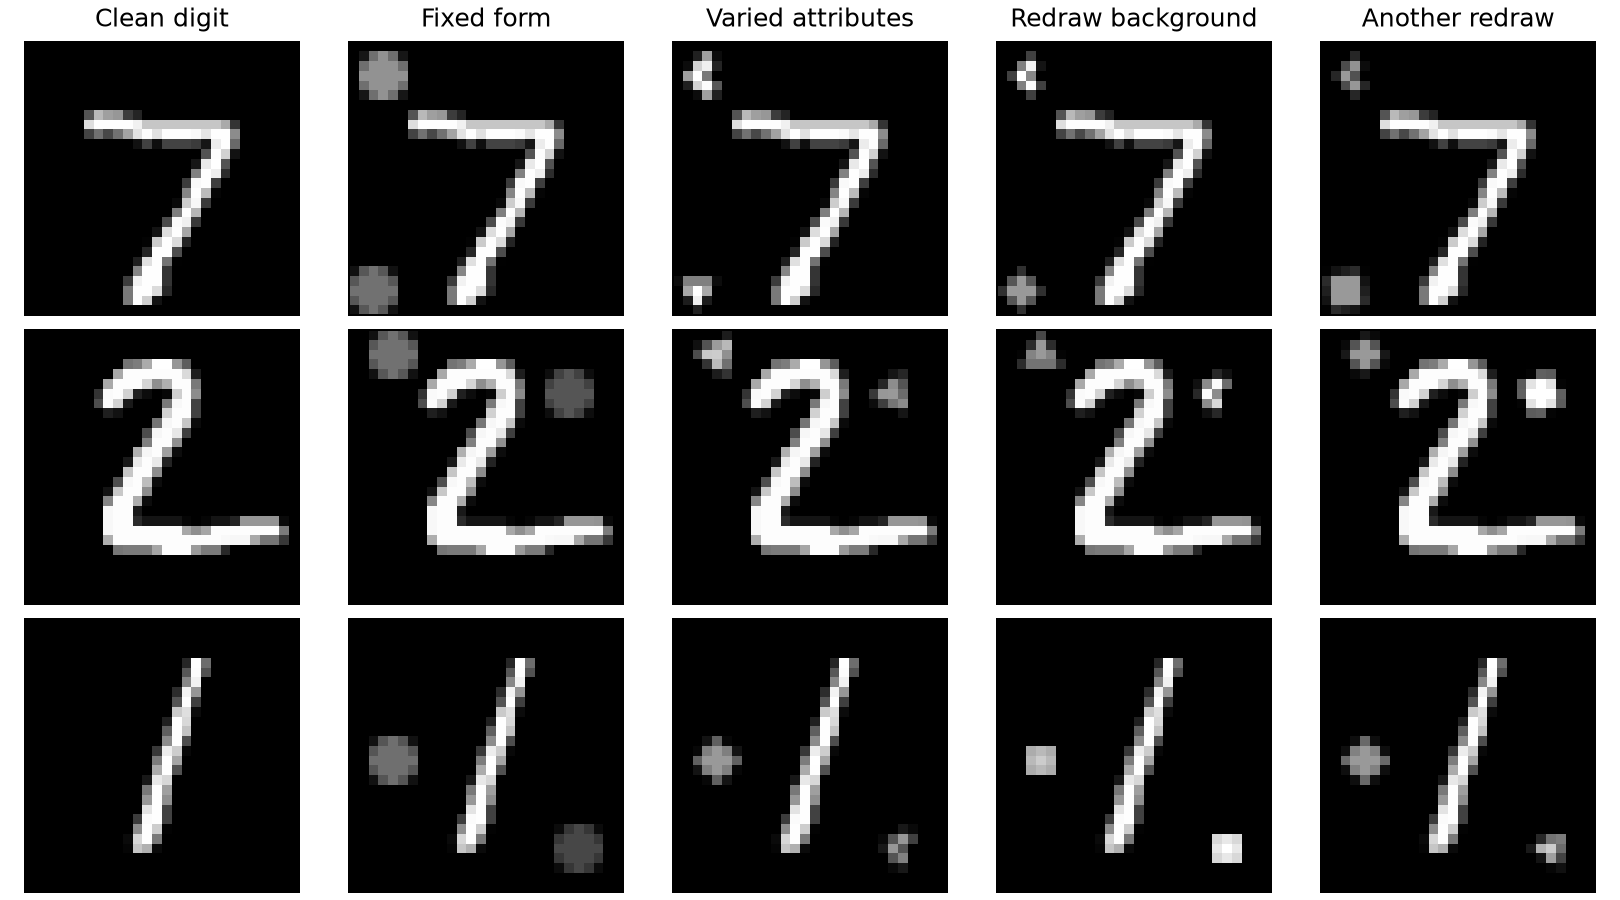
\includegraphics[height=.72\textheight,width=.95\linewidth,keepaspectratio]{../figures/varied.png}
\notefoot{Two symbols per image. All digit pixels stay fixed. The fixed-form control matches every varied symbol's squared pixel energy. There are 96 attribute combinations in the varied bank.}
\end{frame}

\begin{frame}{Does rewarding the background change the outcome?}
\key{Same inputs, two reconstruction targets}\par
Show both models the digit with its random symbols. Reward one for recreating the complete image. Reward the other for recreating the original clean digit.
\par\bigskip
\key{Identify the training stage}\par
Cross the targets during pretraining and clustering. Within each pretrained model, both fine-tuning targets start from exactly the same weights and centers. Also test translation and Gaussian weighting on the varied backgrounds.
\notefoot{Nine conditions, five seeds each. The clean target is privileged information from the synthetic generator and provides a mechanism diagnostic.}
\end{frame}

\begin{frame}{What happens on varied backgrounds?}
\centering\small\setlength{\tabcolsep}{4pt}\begin{tabular}{lrrr}
\toprule
Training condition & In-domain ACC & Clean ACC & Redraw flips\\
\midrule
Clean / full target & 73.96 & 73.96 & ---\\
Fixed form / full target & 65.74 & 68.66 & 2.84\\
Varied / full target & 65.40 & 67.47 & 2.98\\
Varied / clean target & 71.44 & 73.14 & 2.35\\
Varied / translation & 77.63 & 78.68 & 1.89\\
Varied / Gaussian & 69.16 & 70.64 & 2.58\\
\bottomrule
\end{tabular}

\par\bigskip\normalsizeThe clean target recovered 6.04 percentage points of marked accuracy, with a gain in every seed. Fixed-form and varied backgrounds gave similar mean degradation. Translation again gave the highest marked accuracy and lowest redraw flip rate.

\notefoot{Means over five seeds. Background redraws preserve the handwriting. In-domain accuracy uses the test domain matching each row's training inputs.}
\end{frame}
